\documentclass[12pt]{article}%
\usepackage{hyperref}
\usepackage{listings}
\usepackage{color}
\usepackage{multicol}
\usepackage{amsfonts}
\usepackage{fancyhdr}
\usepackage{comment}
\usepackage[a4paper, top=2.2cm, bottom=2.2cm, left=2.2cm, right=2.2cm]%
{geometry}
\usepackage{times}
\usepackage{changepage}
\usepackage{amssymb}
\usepackage{graphicx}%
\newtheorem{theorem}{Theorem}
\newtheorem{acknowledgement}[theorem]{Acknowledgement}
\newtheorem{algorithm}[theorem]{Algorithm}
\newtheorem{axiom}{Axiom}
\newtheorem{case}[theorem]{Case}
\newtheorem{claim}[theorem]{Claim}
\newtheorem{conclusion}[theorem]{Conclusion}
\newtheorem{condition}[theorem]{Condition}
\newtheorem{conjecture}[theorem]{Conjecture}
\newtheorem{corollary}[theorem]{Corollary}
\newtheorem{criterion}[theorem]{Criterion}
\newtheorem{definition}[theorem]{Definition}
\newtheorem{example}[theorem]{Example}
\newtheorem{exercise}[theorem]{Exercise}
\newtheorem{lemma}[theorem]{Lemma}
\newtheorem{notation}[theorem]{Notation}
\newtheorem{problem}[theorem]{Problem}
\newtheorem{proposition}[theorem]{Proposition}
\newtheorem{remark}[theorem]{Remark}
\newtheorem{solution}[theorem]{Solution}
\newtheorem{summary}[theorem]{Summary}
\usepackage{commath}
\usepackage{url} 
\usepackage{hyperref}
\usepackage[style=numeric]{biblatex}
\usepackage{subfig}
\usepackage{minted}
% \usepackage[utf8]{inputenc}
% \usepackage[english]{babel}
\usepackage{esvect}
\addbibresource{reference.bib}


\usepackage{commath}

\newenvironment{proof}[1][Proof]{\textbf{#1.} }{\ \rule{0.5em}{0.5em}}
\usepackage[utf8]{inputenc}

% \usepackage{algorithm}
% \usepackage{algorithmic} %format of the algorithm


% Default fixed font does not support bold face
\DeclareFixedFont{\ttb}{T1}{txtt}{bx}{n}{12} % for bold
\DeclareFixedFont{\ttm}{T1}{txtt}{m}{n}{12}  % for normal

\usepackage{graphics}

% Custom colors
\usepackage{color}
\definecolor{deepblue}{rgb}{0,0,0.5}
\definecolor{deepred}{rgb}{0.6,0,0}
\definecolor{deepgreen}{rgb}{0,0.5,0}

\usepackage{listings}
\newcommand{\Q}{\mathbb{Q}}
\newcommand{\R}{\mathbb{R}}
\newcommand{\C}{\mathbb{C}}
\newcommand{\Z}{\mathbb{Z}}

% Python style for highlighting
\newcommand\pythonstyle{\lstset{
language=Python,
basicstyle=\ttm,
otherkeywords={self},             % Add keywords here
keywordstyle=\ttb\color{deepblue},
emph={MyClass,__init__},          % Custom highlighting
emphstyle=\ttb\color{deepred},    % Custom highlighting style
stringstyle=\color{deepgreen},
frame=tb,                         % Any extra options here
showstringspaces=false            % 
}}

% Python environment
\lstnewenvironment{python}[1][]
{
\pythonstyle
\lstset{#1}
}
{}

% Python for external files
\newcommand\pythonexternal[2][]{{
\pythonstyle
\lstinputlisting[#1]{#2}}}
\usepackage[utf8]{inputenc}
\usepackage{amsmath, nccmath}
\usepackage{geometry}

\usepackage{algorithm}
\usepackage{arevmath}     % For math symbols
\usepackage[noend]{algpseudocode}

\begin{document}

\title{Institute of Robotics,  University of Innopolis}
\author{Computational Intelligence \\ Model Predictive Control }
\date{\today}
\maketitle


We are going to simulate moving a object, typically a point, in 3D space. Assume the system dynamics is described in terms of the LTI (linear time-invariant) state-space model 
\begin{equation} \label{dynamics}
   \begin{aligned}
    x_{k+1} = Ax_k + Bu_k \\
    y_k = Cx_k,
   \end{aligned}
\end{equation} where $x_k \in \mathbb{R}^{n_x}$, $u_k \in \mathbb{R}^{n_u}$, $y_k \in \mathbb{R}^{n_y}$, and A and B are given by:
\begin{equation} \label{eq1}
   A = \begin{bmatrix}
1 & 0 & 0\\ 
0 & 1 & 0\\ 
0 & 0 & 1\\ 
\end{bmatrix}, \quad B =  \begin{bmatrix}
1 & 0 & 0\\ 
0 & 1 & 0\\ 
0 & 0 & 1\\ 
\end{bmatrix}.
\end{equation}$x_k$ and $u_k$ describe position and velocity, respectively in x,y, and z direction in 3D space at time index i.e., k. $-6\leq x_k \leq 6$ and $-0.1\leq u_k \leq 0.1$ are the constraints that are being applied on the point when moving through space. Let $x_{init}$ be the start position where the point is moved, and $x_{ref}$ be the target position. The objective is to formulate the preceding problem as an optimization problem in which an optimal control policy should be calculated at each time instance solving the following quadratic optimization problem and apply the first potion to the system. 

\begin{figure}[H]
    \begin{center}
    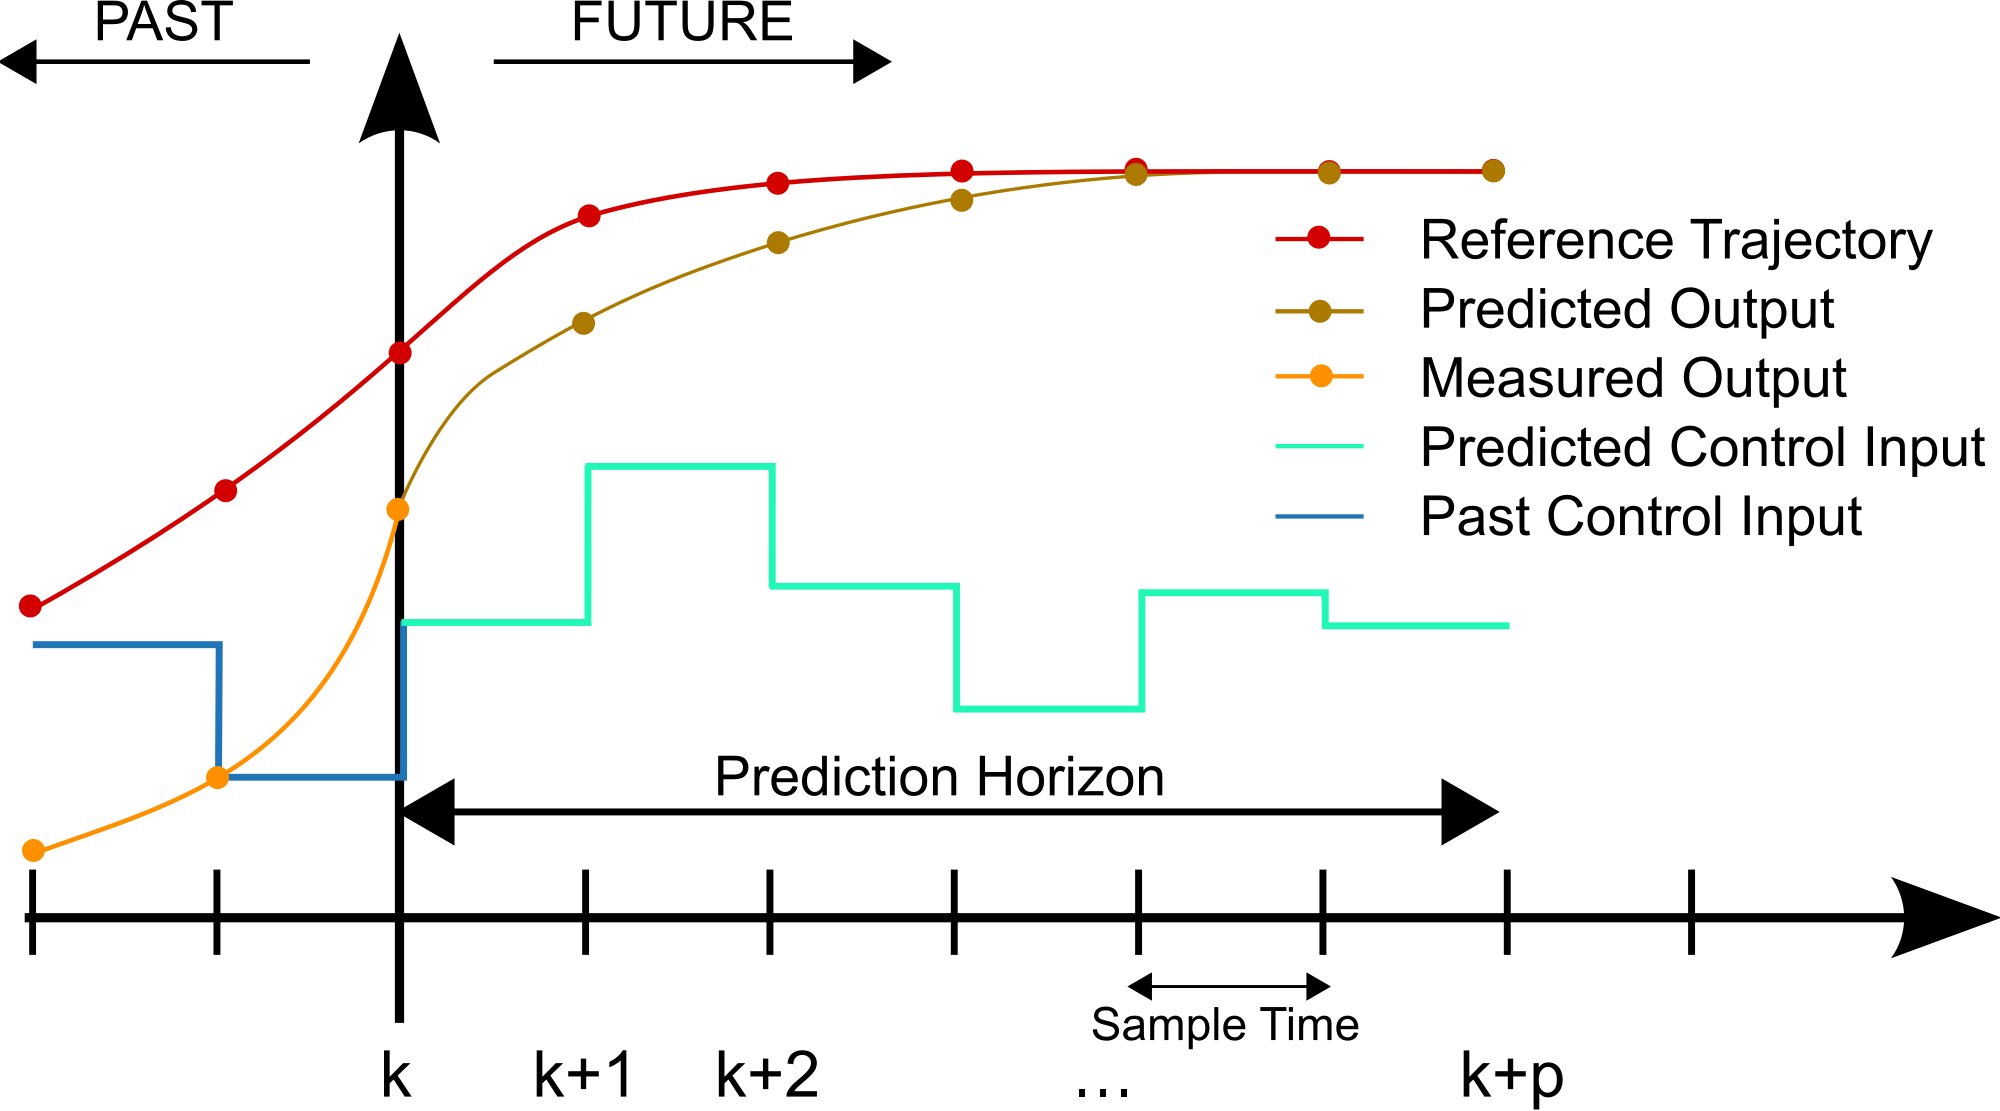
\includegraphics[width=13cm]{mpc.png}
    \caption{Model Predictive Control in a nutshell\cite{mpc1}}\label{f:mpc}
    \end{center}
\end{figure}

\begin{equation}\label{mpc_1}
\begin{aligned}
\min_{\mathbf{u}, \mathbf{x}} \quad & \sum_{k=0}^{n-1} (x_k-x_{ref})^T Q (x_k-x_{ref}) + u_k^T R u_k + (x_n-x_{ref})^T Q_n (x_n-x_{ref})   \\
\textrm{s.t.} \quad & x_{k+1} = A x_k + B u_k \\ 
 & x_{\rm min} \le x_k  \le x_{\rm max} \\
 & u_{\rm min} \le u_k  \le u_{\rm max} \\
 & x_0 = x_{init},
\end{aligned}
\end{equation} where $Q_n = Q = R = diag(1,1,1)$. You may decide a value for N appropriately. Further instructions are provided in the skeleton code. Expected output should be similar to Fig.\ref{f:simulated_result} for $x_{init} = <5,5,1>$ and $x_{ref} =,-2,-3.,5.>$

\begin{figure}[H]
    \begin{center}
    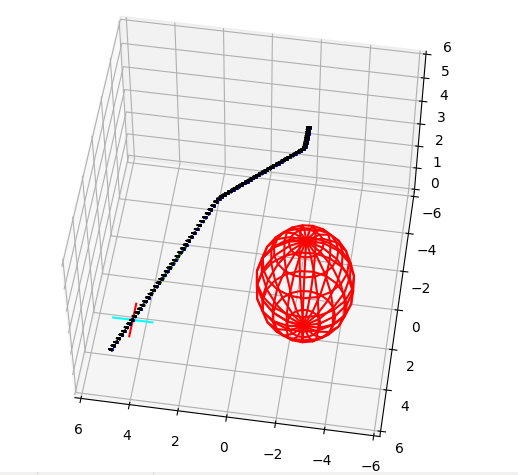
\includegraphics[width=13cm]{simulated_result.png}
    \caption{}\label{f:simulated_result}
    \end{center}
\end{figure}

In order to simulate and verify your implementation, you may use the following code in which you have to stack state of the system at each time instance, i.e.,  stacked states are in the form ($n_s$, 3) matrix where $n_s$ is the number tries solver used to get to the $x_{ref}$. For $n_s$ times, predicted trajectory describes by a matrix with dimension ($n_s$, 21, 3). Yet, simulator is required it is be ($n_s$, 21, 4). You may have to to add zero column to the original matrix, i.e., $prediction\_horizon\_poses$, before constituting as input to the the simulator. 


Comment on how can we incorporate a set of static obstacles as a new constraints set and heading of the moving object.    

\begin{minted}
[frame=lines, framesep=2mm, baselinestretch=1.2,]
{python}
df = np.array(current_state)
quadcopter = QuadCopter() 
def control_loop(i):
    state = np.array(df[i])
    return quadcopter.world_frame(np.append(state, 0)
                    , prediction_horizon_poses[i])
    
obs_map = np.array([[-2.5, 1.5, 2, 2]])
quadcopter.plot_quad_3d(control_loop, obs_map)
\end{minted}

\printbibliography
\end{document}